\documentclass[12pt]{article}
\usepackage[utf8]{inputenc}
\usepackage{graphicx}
\usepackage{subcaption}
\usepackage{amsmath} 
\usepackage{fancyhdr} 
\usepackage{geometry} 
\usepackage{dirtytalk} 
\usepackage[english]{babel}
\usepackage{csquotes}
\usepackage{hyperref}
\usepackage{listings}
\lstset{
    language=C,
    basicstyle=\ttfamily, 
    numberstyle=\tiny,
    frame=single,
    breaklines=true,
}

\begin{document}
\begin{titlepage}
\begin{center}
    
\includegraphics[width=0.3\textwidth]{image.png} \\[0.2cm]
    
    \textbf{MINISTRY OF EDUCATION, CULTURE AND RESEARCH 
OF THE REPUBLIC OF MOLDOVA} \\[0.3cm]
    
    \textbf{Technical University of Moldova 
Faculty of Computers, Informatics and Microelectronics 
Department of Software and Automation Engineering} \\[2cm]
    
    \textbf{Postoronca Dumitru FAF-233}\\[0.5cm]
    
    \Huge \textbf{Report} \\[0.5cm]
    
    \large Laboratory work n.2 \\[0.5cm]
    
    \textbf{of CS} \\[3cm]
    
    \begin{flushright}
        \textit{Checked by:} \\
        \textbf{A. Zaica}, \textit{university assistant} \\
        DISA, FCIM, UTM
    \end{flushright}
    
    \vfill
    
    Chișinău -- 2025
\end{center}
\end{titlepage}


\newpage
\setcounter{page}{1}
\pagestyle{fancy}
\fancyhf{}
\rhead{\thepage}
\lhead{FAF-233 Postoronca Dumitru ; Laboratory Work №1}

\section{Purpose of the Laboratory Work}
The purpose of this laboratory was to study the concept of frequency analysis as a method of 
cryptanalysis. Frequency analysis is one of the oldest techniques for breaking classical ciphers 
and is based on the observation that letters in natural languages appear with characteristic 
frequencies. For example, in the English language, the letters \texttt{E}, \texttt{T}, \texttt{A}, 
and \texttt{O} occur most often, while letters such as \texttt{Z}, \texttt{Q}, and \texttt{X} 
are much less frequent. By comparing the distribution of characters in the ciphertext with the 
expected distribution in English, it is possible to make informed guesses about the substitutions 
and progressively decrypt the message.

\section{Strategy Used}
To carry out this task, I first analyzed the frequencies of the letters in the given encrypted text 
and compared them with the known frequency distribution of English letters. Based on this 
comparison, I made initial assumptions about which ciphertext letters corresponded to which 
plaintext letters.  

To simplify the decryption process, I developed a small interactive website. This tool allowed me 
to dynamically replace ciphertext letters with my assumptions, observe the updated text in real 
time, and iteratively refine the mapping. This approach significantly sped up the process of 
testing hypotheses and correcting mistakes.

\section{Decryption Process}
The decryption process was iterative and consisted of the following steps:

\begin{enumerate}
    \item Calculate the frequency distribution of the ciphertext characters.
    \item Match the most frequent symbols with the common English letters such as \texttt{E}, 
    \texttt{T}, and \texttt{A}.
    \item Dynamically replace characters using the developed website, checking if meaningful words 
    begin to form.
    \item Refine the mappings step by step until the majority of the text became readable and the 
    intended plaintext was reconstructed.
\end{enumerate}

\begin{figure}
    \centering
    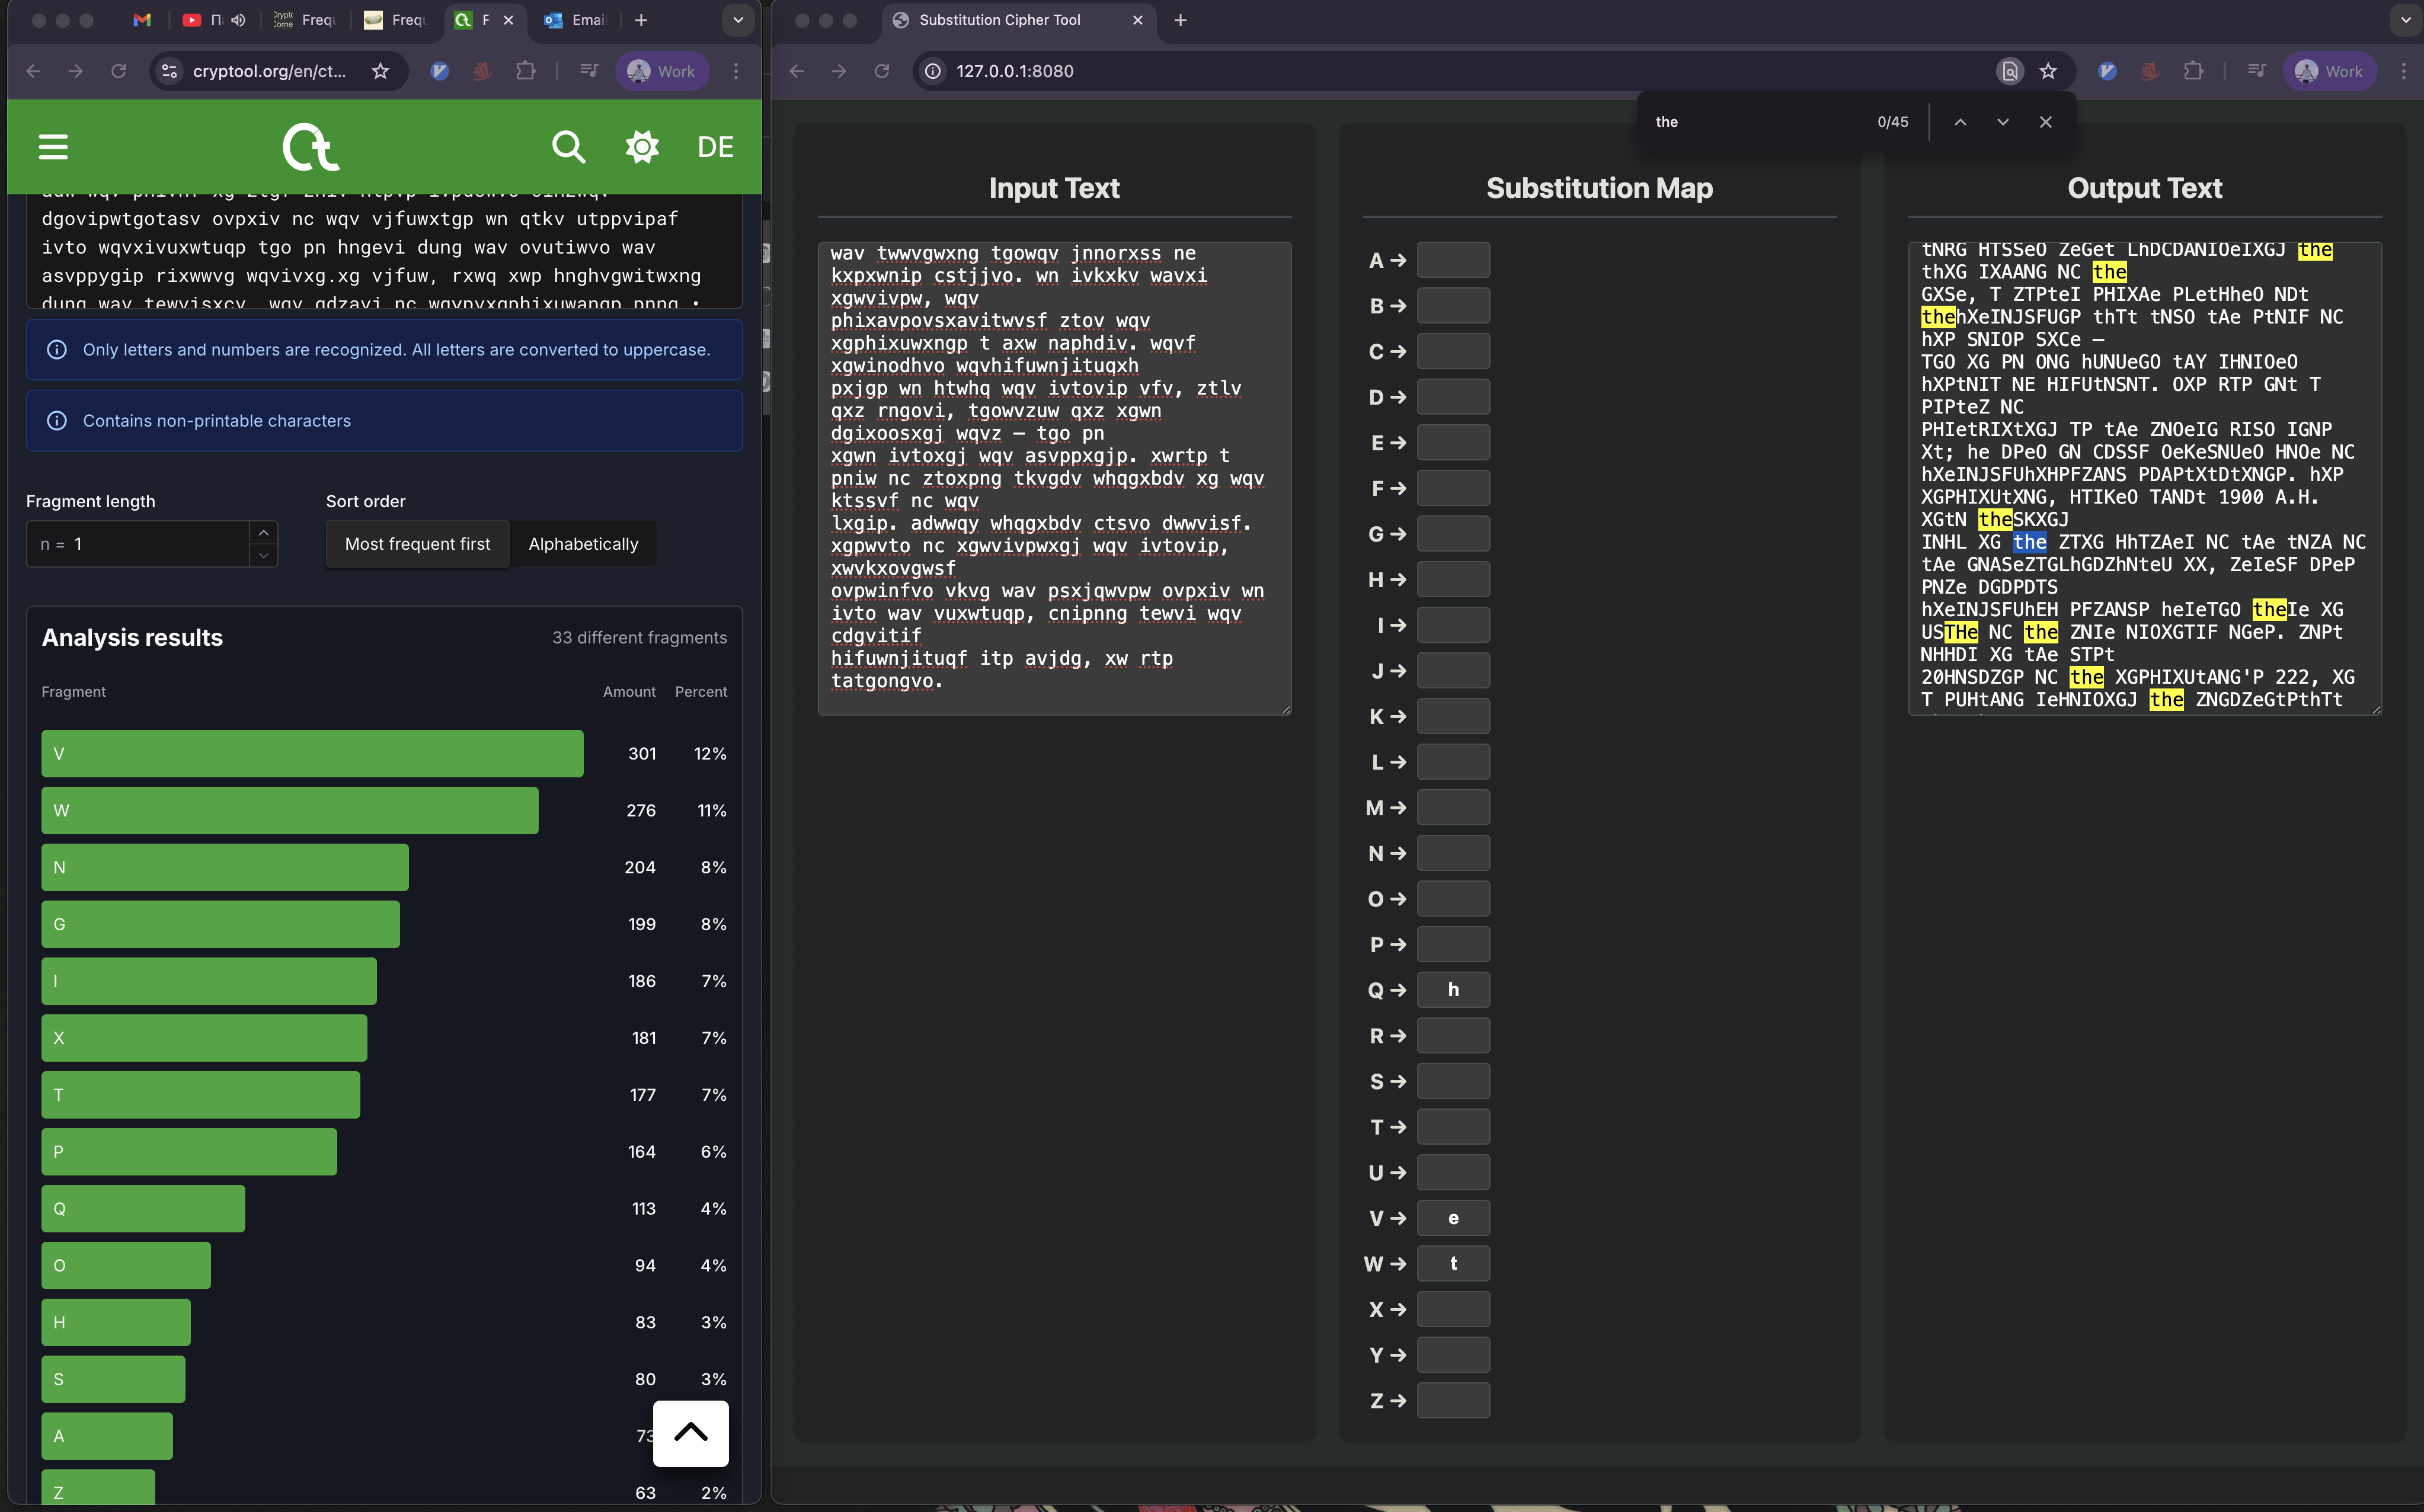
\includegraphics[width=0.7\textwidth]{frequency.png}
    \caption{Progress of the decryption process using the interactive replacement tool.}
\end{figure}
\begin{figure}
    \centering
    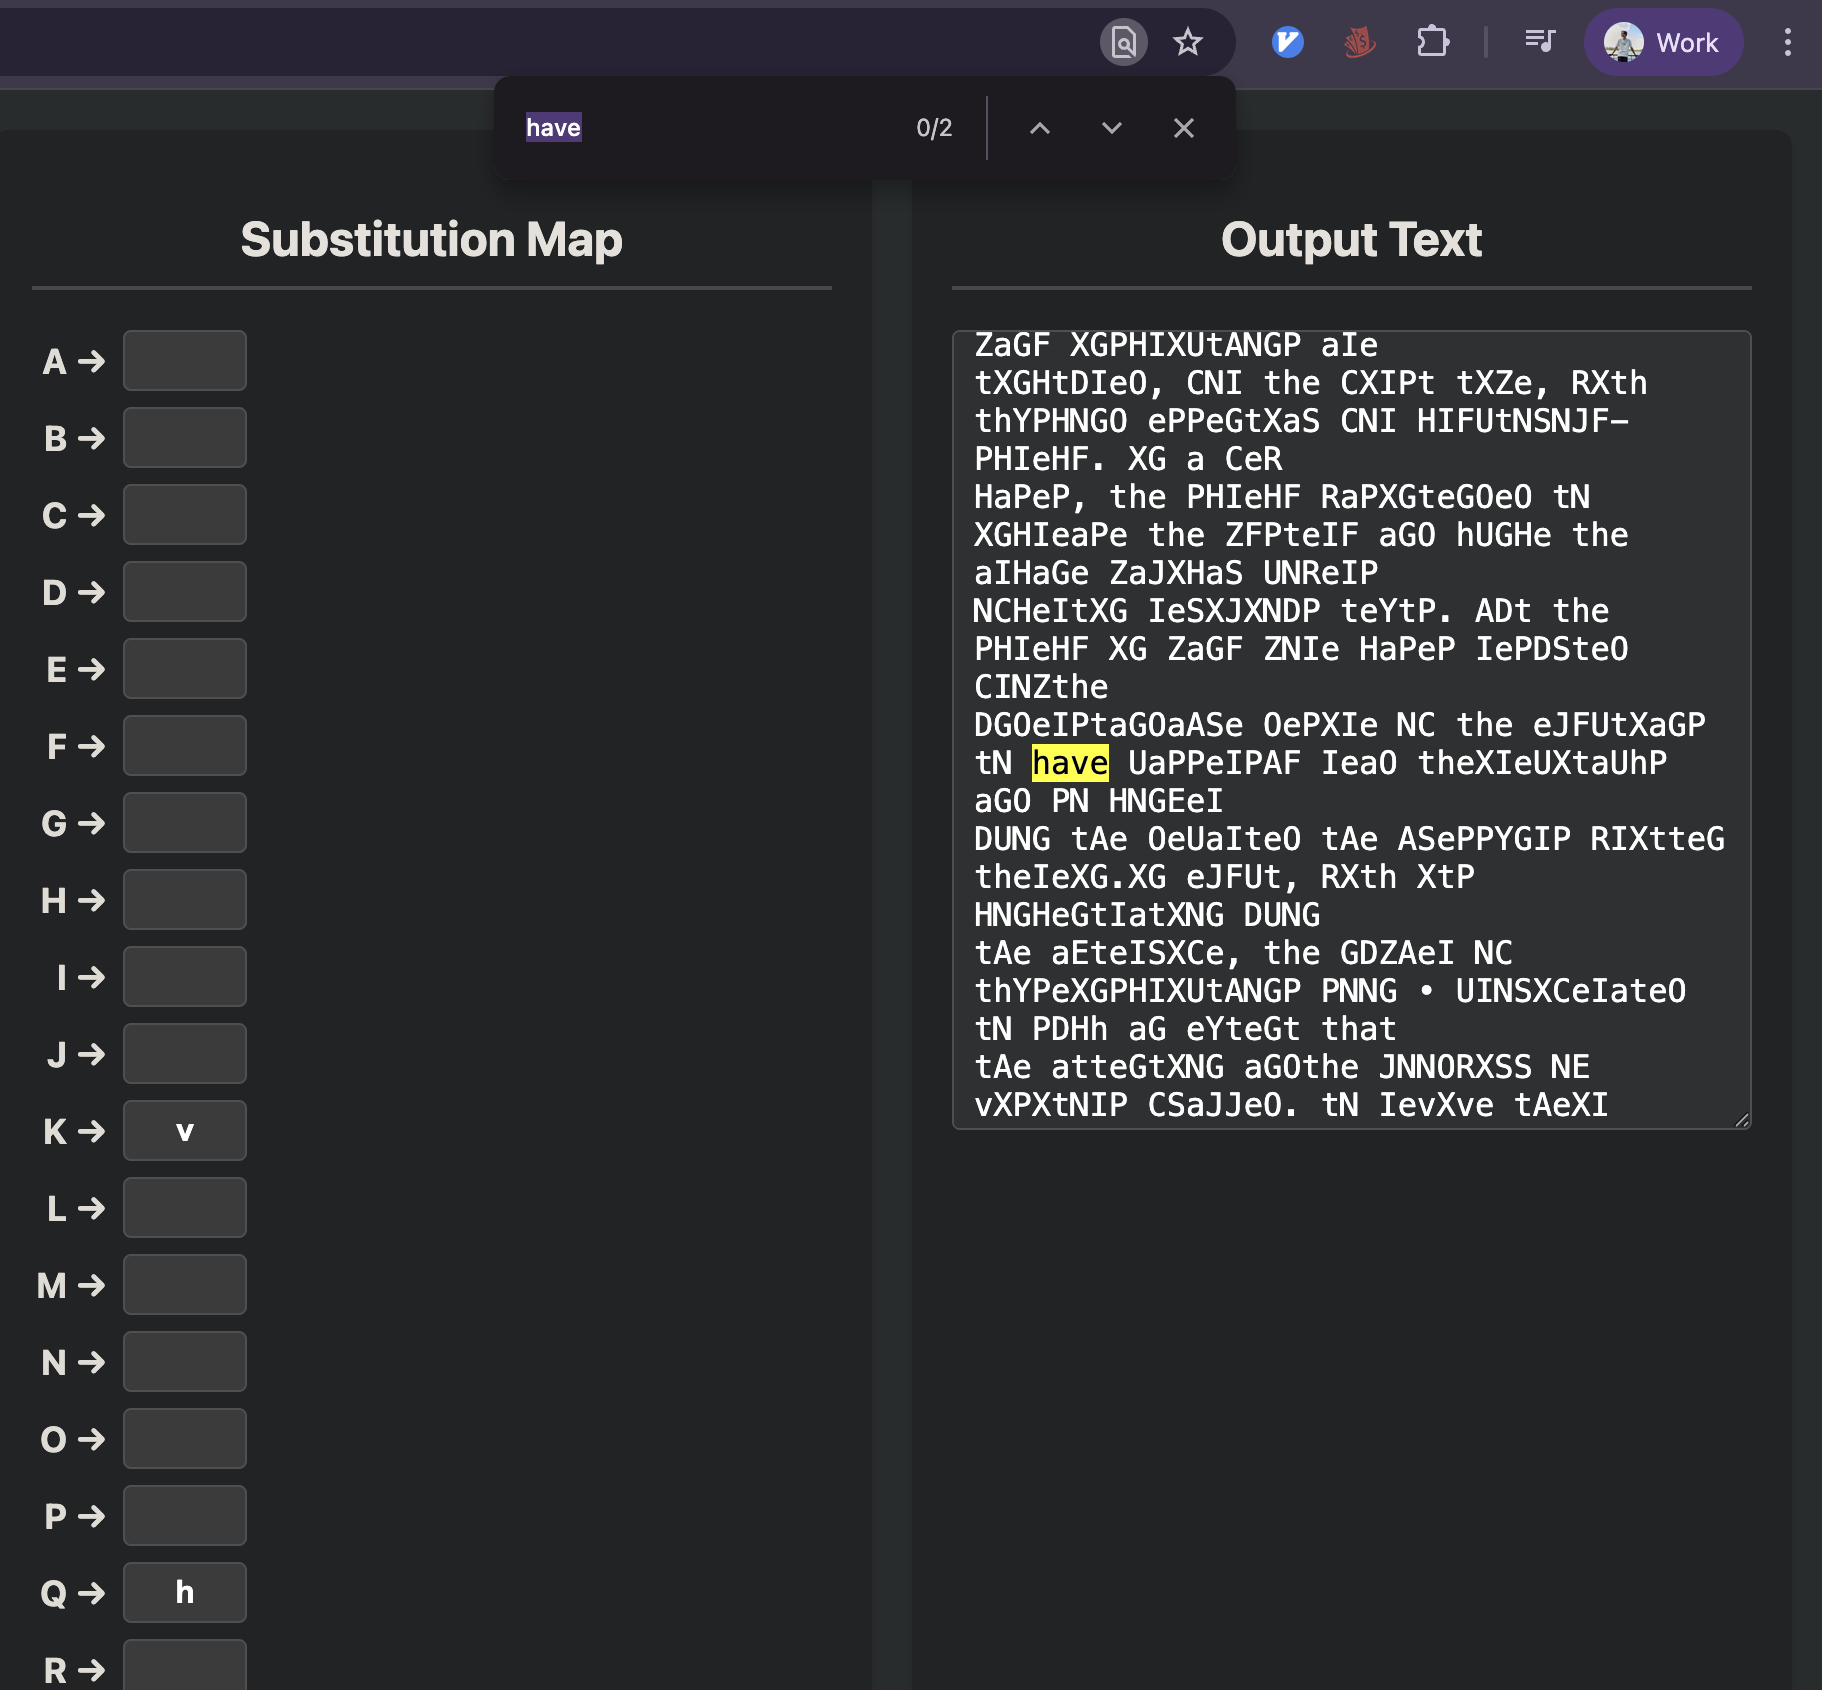
\includegraphics[width=0.7\textwidth]{step_1.png}
    \caption{Breaking down the first words}
\end{figure}
\begin{figure}
    \centering
    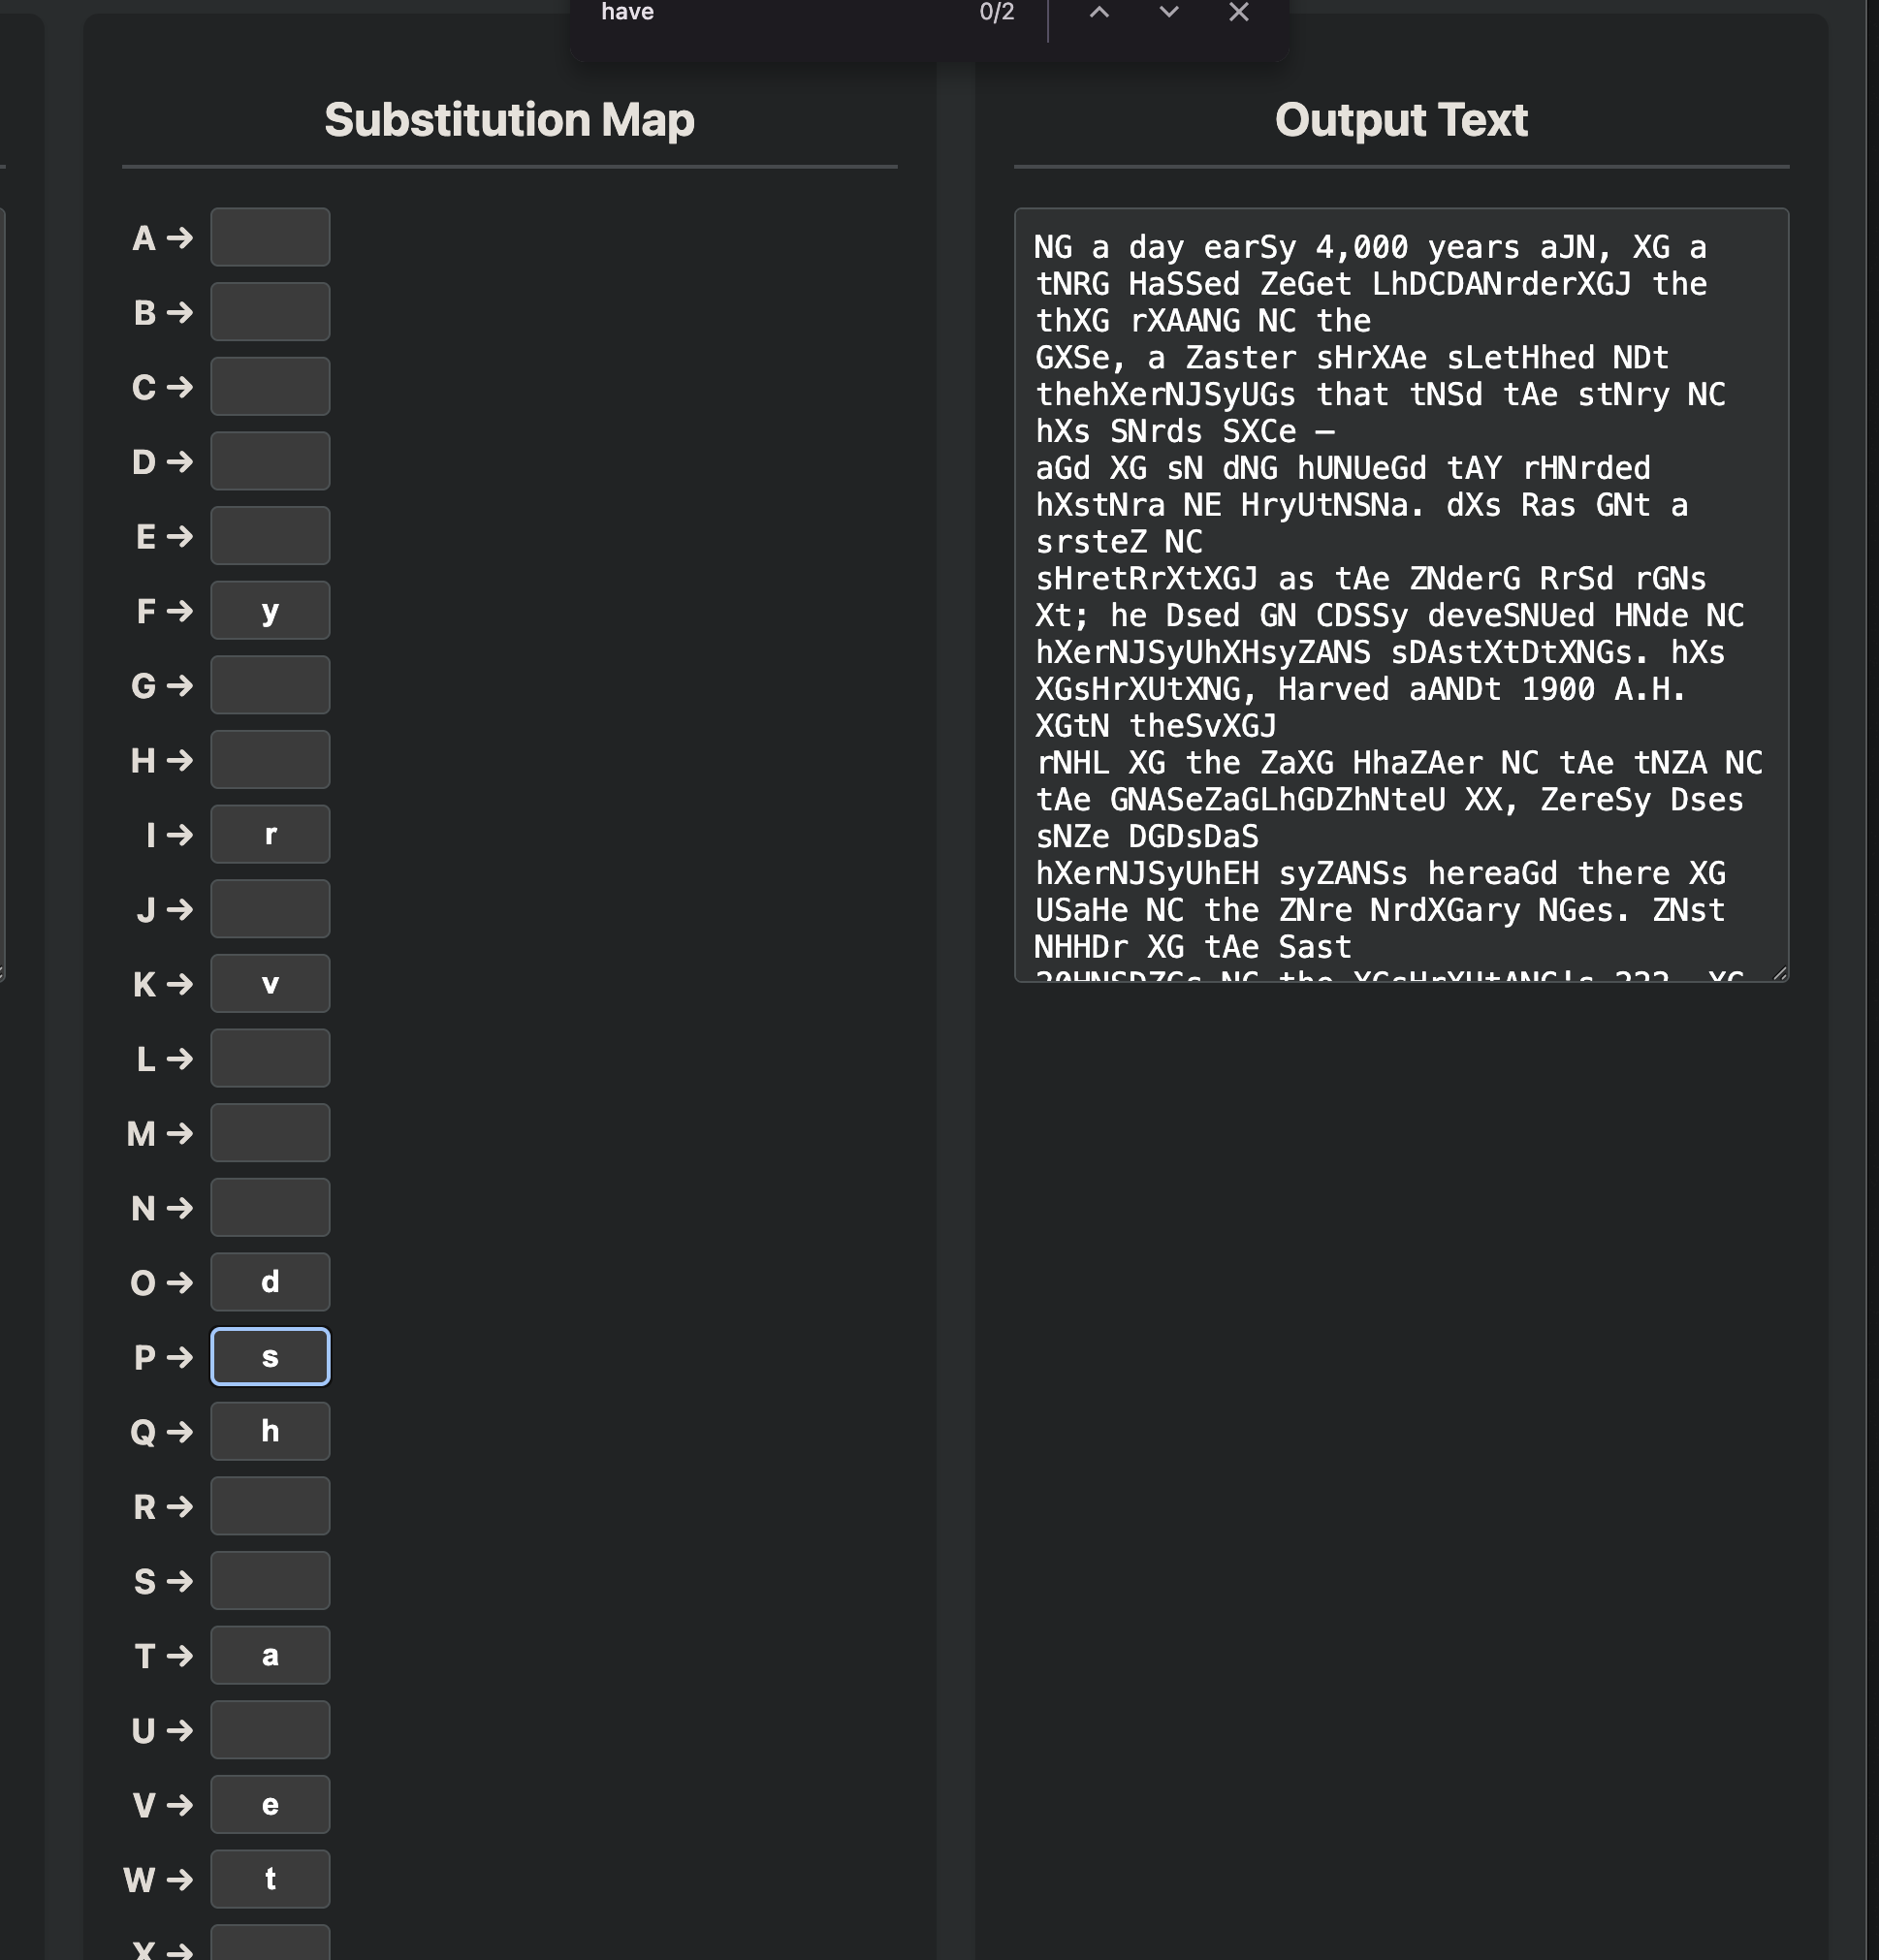
\includegraphics[width=0.7\textwidth]{step_2.png}
    \caption{Third of the letters are known}
\end{figure}
\begin{figure}
    \centering
    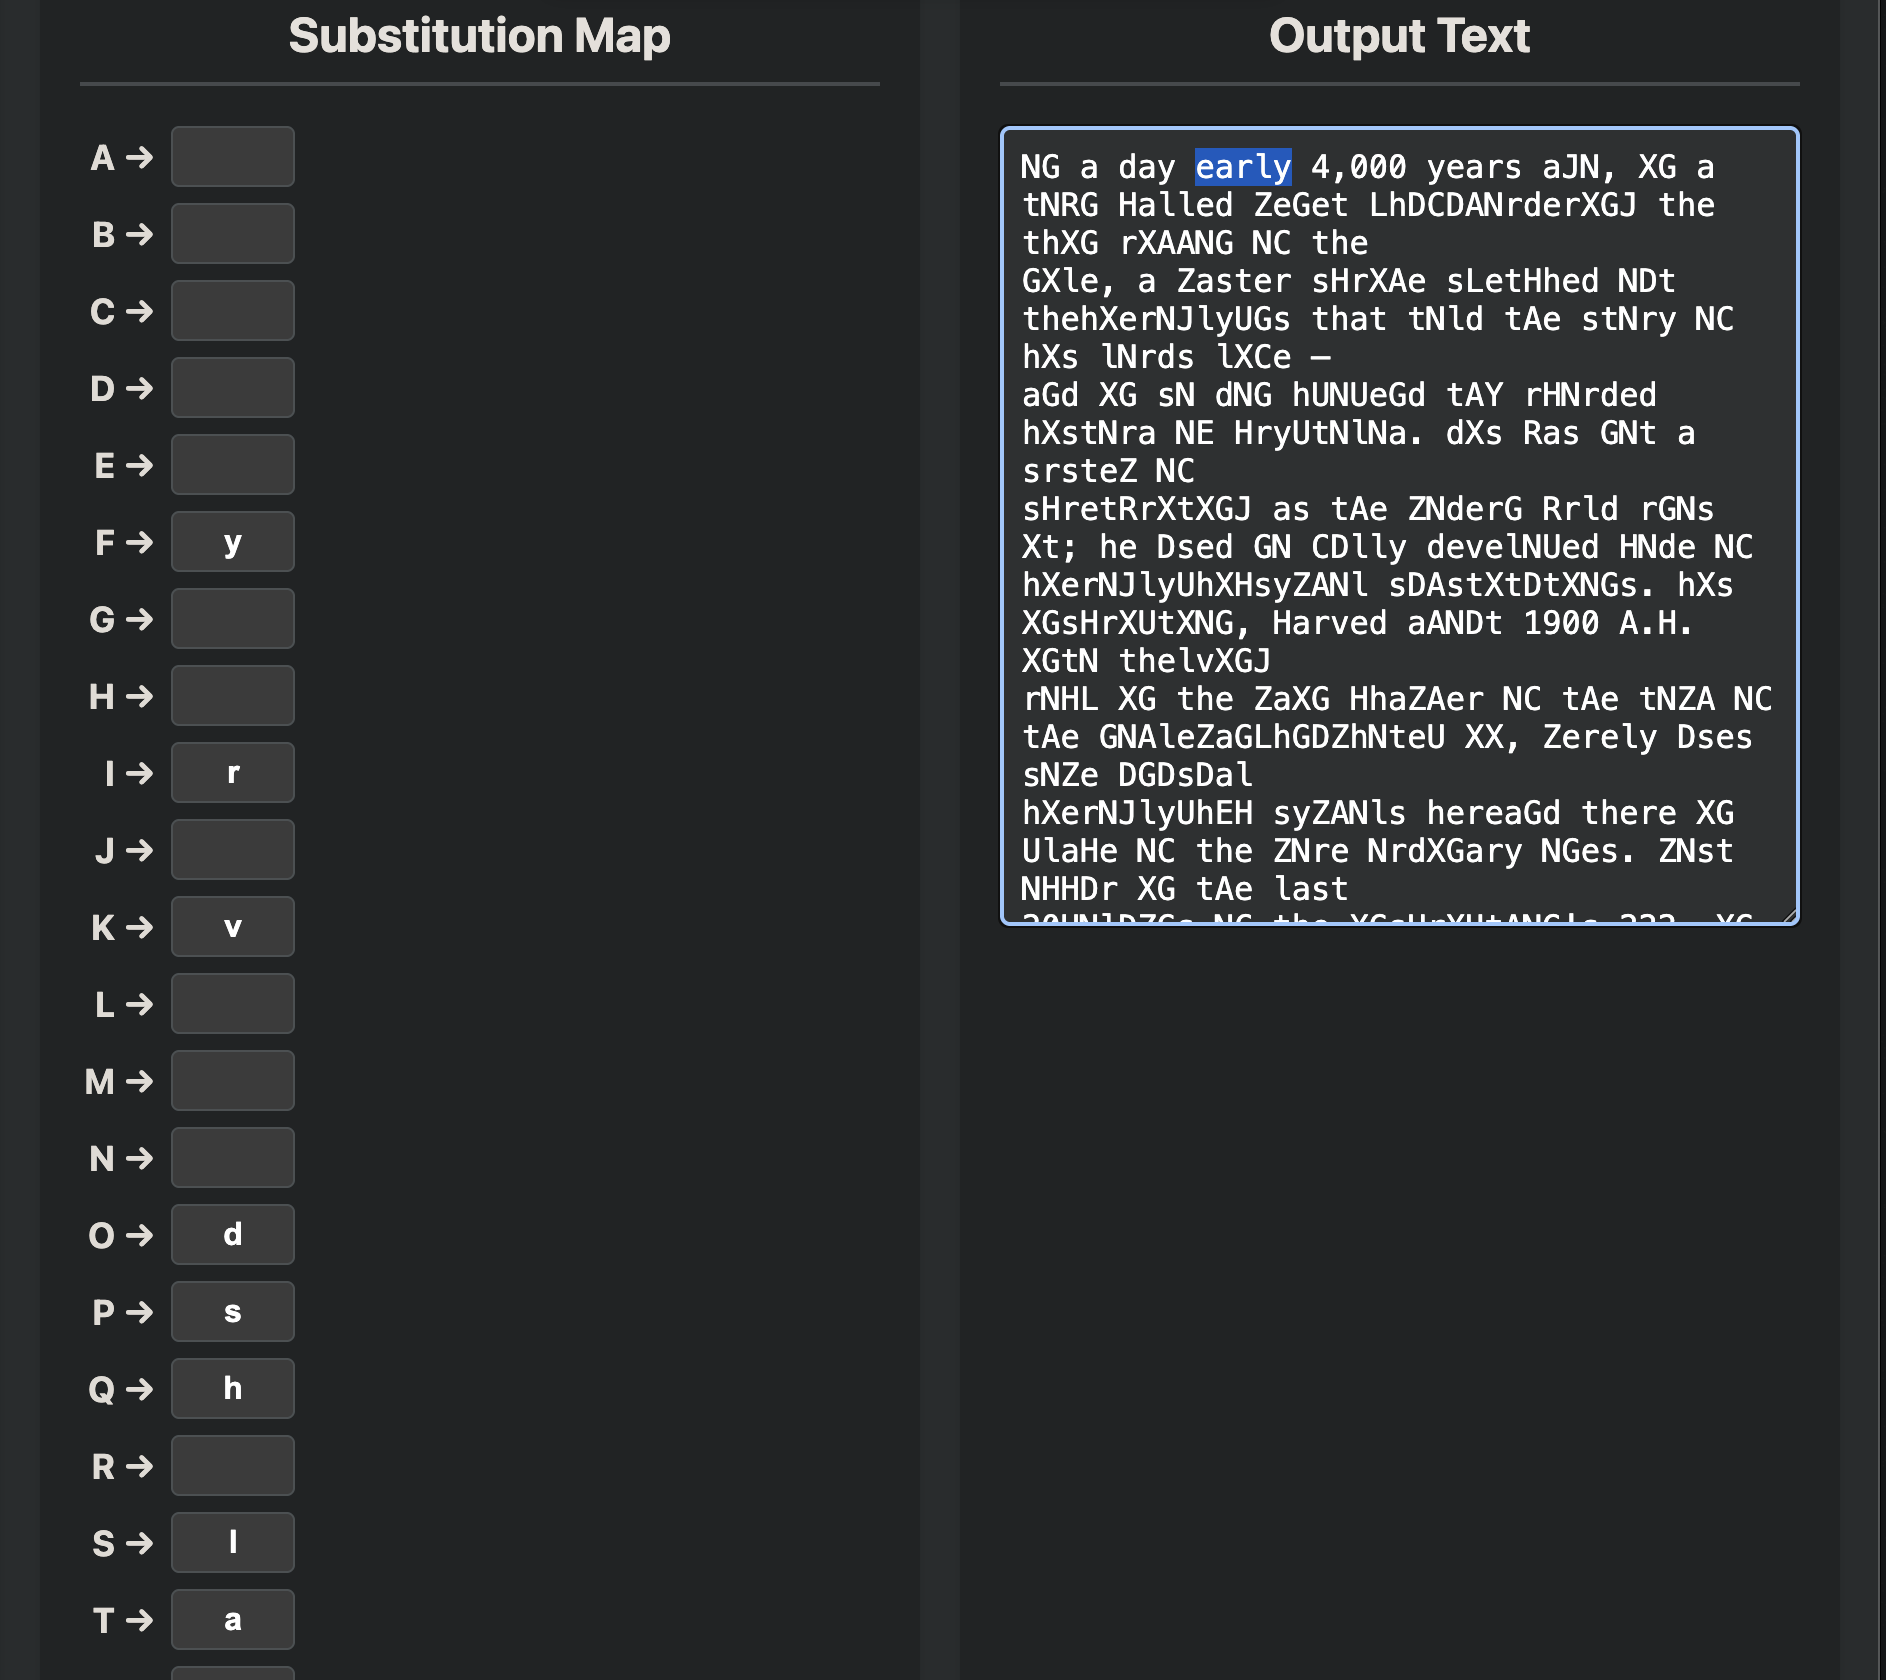
\includegraphics[width=0.7\textwidth]{step_3.png}
    \caption{}
\end{figure}
\begin{figure}
    \centering
    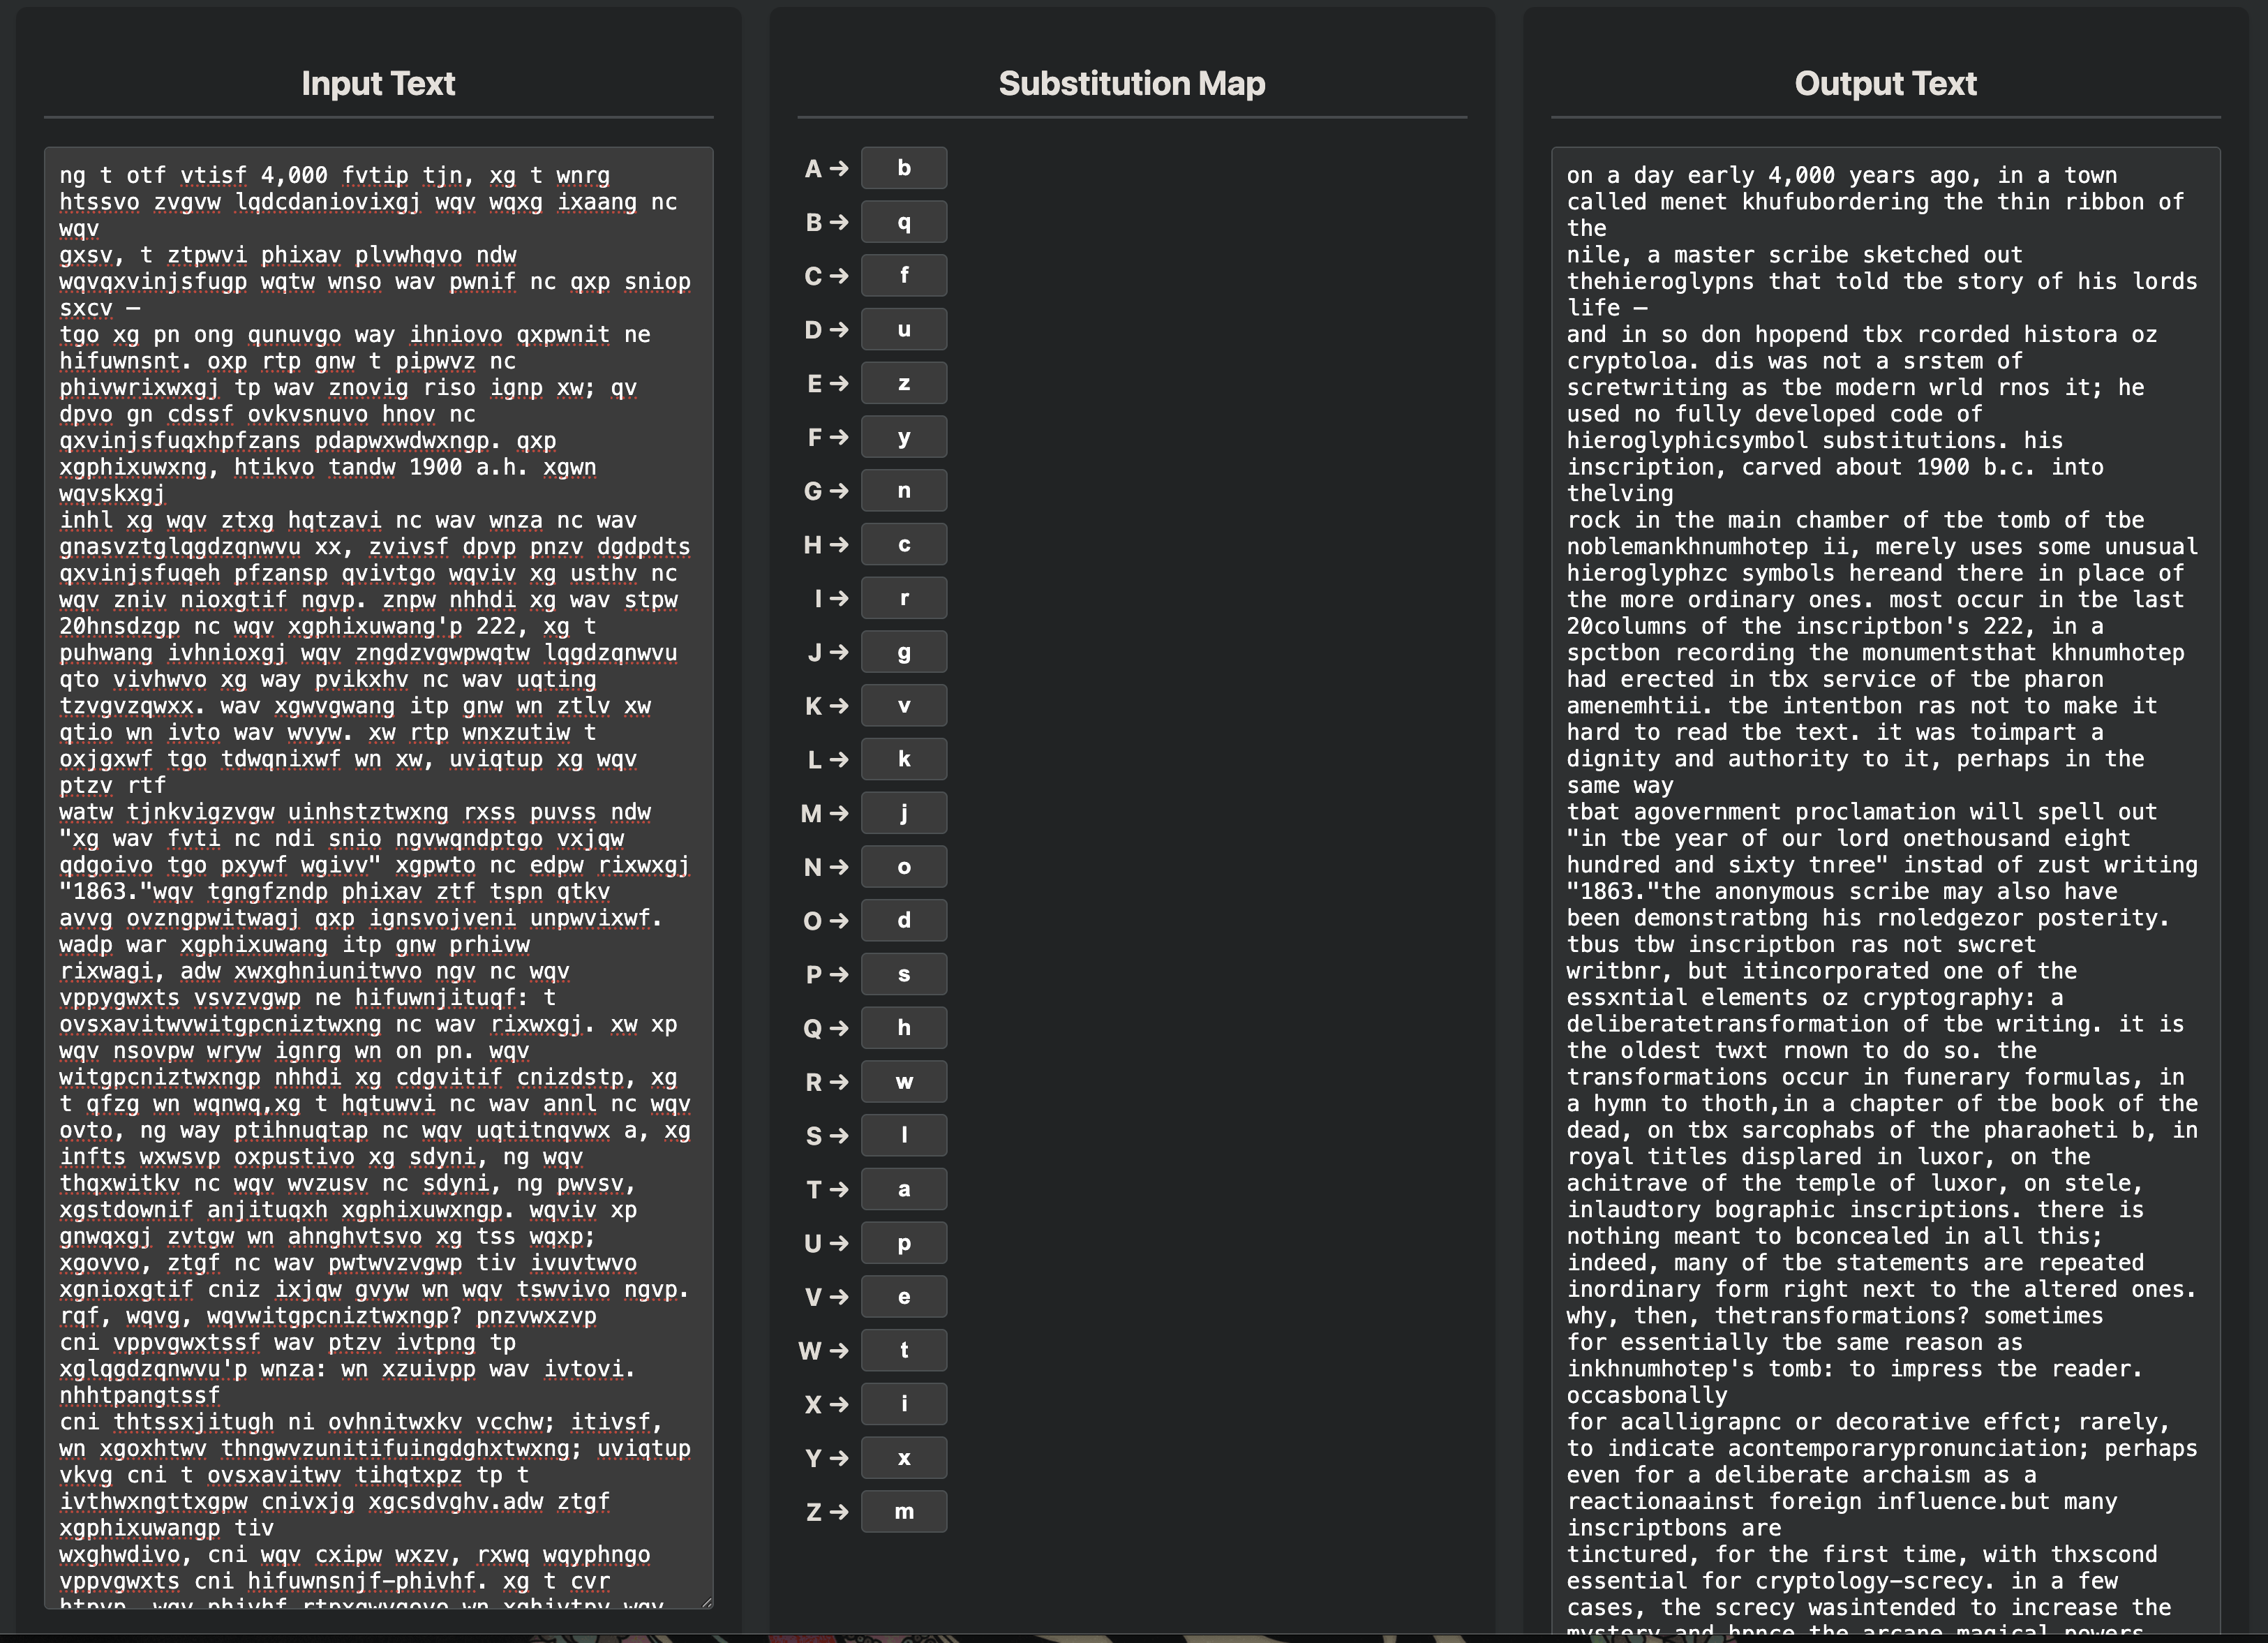
\includegraphics[width=0.7\textwidth]{final_result.png}
    \caption{text is fully cracked}
\end{figure}

The use of an interactive visualization tool proved to be highly effective, as it allowed quick 
adjustments and an intuitive workflow for breaking the cipher.



\clearpage
\section{Conclusion}

This laboratory work provided practical experience with one of the fundamental techniques of 
classical cryptanalysis — frequency analysis. By comparing the distribution of letters in the 
ciphertext with the expected frequencies of letters in the English language, I was able to 
gradually reconstruct the original message.  

The use of an interactive website for testing assumptions greatly simplified the process, making 
it possible to quickly validate or discard hypotheses and progressively refine the decryption.  
Through this exercise, I gained a deeper understanding of the weaknesses of substitution ciphers 
and why they are considered insecure by modern standards. At the same time, the laboratory 
highlighted the power of statistical methods in cryptanalysis and their historical importance in 
the development of cryptography.
\end{document}
